\chapter{Программный комплекс для интерактивной визуализации сложных сцен конструктивно-блочной геометрии на графических процессорах и его экспериментальное исследование} \label{chapt3}

Данная глава посвящена экспериментальному исследованию разработанного комплекса и отвечает следующим целям:
\begin{itemize}
  \item Представить описание состава и структуры разработанного программного комплекса для интерактивной визуализации сложных сцен конструктивно-блочной геометрии на графических процессорах, который реализует положения главы 2 с использованием инструментов программирования параллельных графических архитектур.

  \item Экспериментально проверить корректность моделирования глобального освещения в сцене путем сравнения результатов моделирования с эталонными изображениями.

  \item Дать оценку производительности программного комплекса, а также оценку эффективности предложенных решений относительно аналогов.
\end{itemize}

\section{Состав и структура программного комплекса для интерактивной визуализации сложных сцен конструктивно-блочной геометрии на графических процессорах}

\subsection{Высокопроизводительные свободно распространяемые библиотеки нижнего уровня}

В разработанном программном комплексе активно применяются следующие свободно распространяемые библиотеки:

\begin{itemize}
    \item Eigen [http://eigen.tuxfamily.org]. Библиотека шаблонов на языке C++ для линейной алгебры. Характеризуется универсальностью, высоким уровнем производительности, лаконичностью программных интерфейсов (вектора и матрицы) и поддержкой многих компиляторов. Высокое быстродействие достигается посредством применения SIMD-расширений ЦПУ и техник метапрограммирования (таких как Expression Templates). Библиотека доступна с исходным кодом по лицензиям LGPL3 и GPL2.
    \item Boost [http://www.boost.org]. Собрание библиотек, расширяющих язык C++ подобно STL (Standard Template Library). Библиотеки Boost ускоряют массу задач прикладного программирования, предоставляя типичные алгоритмы, контейнеры данных, «умные указатели», примитивы многопоточного программирования и многое другое. Данные библиотеки доступны с исходным кодом по лицензии Boost Software License.
    \item Qt [http://qt-project.org]. Кросс-платформенный инструментарий разработки ПО на языке C++. Содержит основные классы, которые могут потребоваться при разработке прикладного программного обеспечения, включая элементы графического интерфейса пользователя. Инструментарий Qt является полностью объектно-ориентированным и поддерживает технологию компонентного программирования. Библиотека доступна с исходным кодом по лицензиям GPL3 и LGPL.
    \item GLog [http://code.google.com/p/google-glog]. Вспомогательная библиотека на языках C/C++, которая позволяет записывать в журнал приложения указанные разработчиком события (application-level logging). Данный функционал позволяет упростить отладку и выявление проблем. Библиотека распространяется с исходным кодом по лицензии New BSD.
    \item GLEW [http://sourceforge.net/projects/glew]. Мультиплатформенная библиотека на языке C для работы с расширениями OpenGL (поддерживает версию 4.3). Доступна с исходным кодом по лицензиям BSD и MIT.
    \item GLFW [http://www.glfw.org/index.html]. Мультиплатформенная библиотека на языке C для создания контекста OpenGL и управления вводом, включая клавиатуру, мышь и джойстик. Распространяется с исходным кодом по лицензии zlib/libpng.
\end{itemize}

Наряду с указанными библиотеками в разработанном комплексе применяются инструменты программирования графических процессоров предоставляемые интерфейсом программирования OpenGL.

\subsection{Структура программного комплекса и состав его библиотек прикладных программ}

Разработанный программный комплекс состоит из набора модулей, которые основаны на перечисленных выше базовых библиотеках (рис. \ref{fig:arch}). На нижнем слое функциональности расположена библиотека Graphics. Библиотека Graphics отвечает за поддержку типовых задач программирования 3D графики OpenGL, включая управление виртуальными камерами и устройствами ввода, загрузку изображений, настройку шейдерных программ и буферов кадров. Основная функциональность программного комплекса содержится в библиотеках \textit{CSG} и \textit{Renderer}. Библиотека \textit{CSG} реализует рассмотренное в главе 2 иерархическое представление CSG сцены, а также описания материалов и источников света. Библиотека \textit{Renderer} реализует программный конвейер трассировки лучей (путей). Верхний слой функциональности представлен библиотеками \textit{Convert} и \textit{GUI}, которые отвечают за импорт моделей CSG сцен (во внутренний формат системы) и содержат некоторые элементы графического интерфейса Qt (многорежимное окно визуализации с возможностью переключения между различными режимами визуализации).

\begin{figure}[ht]
  \centering
  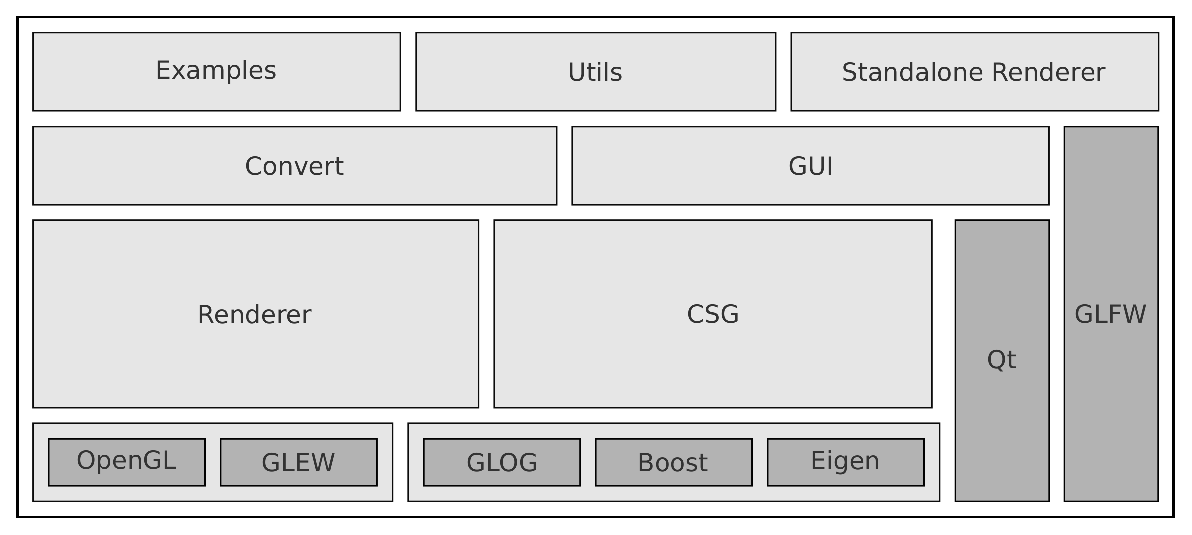
\includegraphics [scale=0.8] {arch}
  \caption{Основные компоненты разработанного программного комплекса}
  \label{fig:arch}
\end{figure}

На основе верхнего уровня функциональности разрабатываются различные клиентские программы, включая тестовые и демонстрационные приложения, а такде специализированные системы визуализации. На данный момент разработан автономный визуализатор с возможностью редактирования CSG сцены.

В совокупности разработанные библиотеки и приложения содержат свыше 50 файлов программного кода (более 10 000 строк).

\section{Исследование производительности программного комплекса} \label{sect_results}

Оценки производительности для данного исследования были получены на графических процессорах: NVIDIA GeForce GTX 680, AMD Radeon HD 7870 и Intel HD 4000. Измерения проводились при отрисовке в окно размером 1280 x 720. Первая сцена для тестирования предложенного алгоритма представляет собой CSG модель города (см. Рисунок \ref{fig:results_city}). Во всех вариантах сцена составлена как одно CSG дерево (схожие элементы добавлены с помощью операции объединения). В простейшей конфигурации (в) модель состоит из 3385 примитивов. Более сложные варианты сцены (г), (д) и (е) состоят из 86К, 343К и 987К примитивов соответственно. Рисунок (б) представляет собой пример сложного для альтернативных решений ракурса, с большим числом слоёв глубины. Сцена «Город», представленная в трёх вариантах позволяет проанализировать зависимость производительности предложенного алгоритма от сложности CSG модели. Для каждого графического процессора результаты представлены в виде двух столбцов (см. Таблицу \ref{tbl:timings}): левый соответствует измеренному значению величины отображённых кадров в секунду (Frames Per Second, FPS) без пространственной оптимизации дерева ($-$), правый содержит значения, полученные с выполненной пространственной оптимизацией ($+$).

\begin{figure}[ht]
  \begin{minipage}[ht]{0.49\linewidth}\centering
    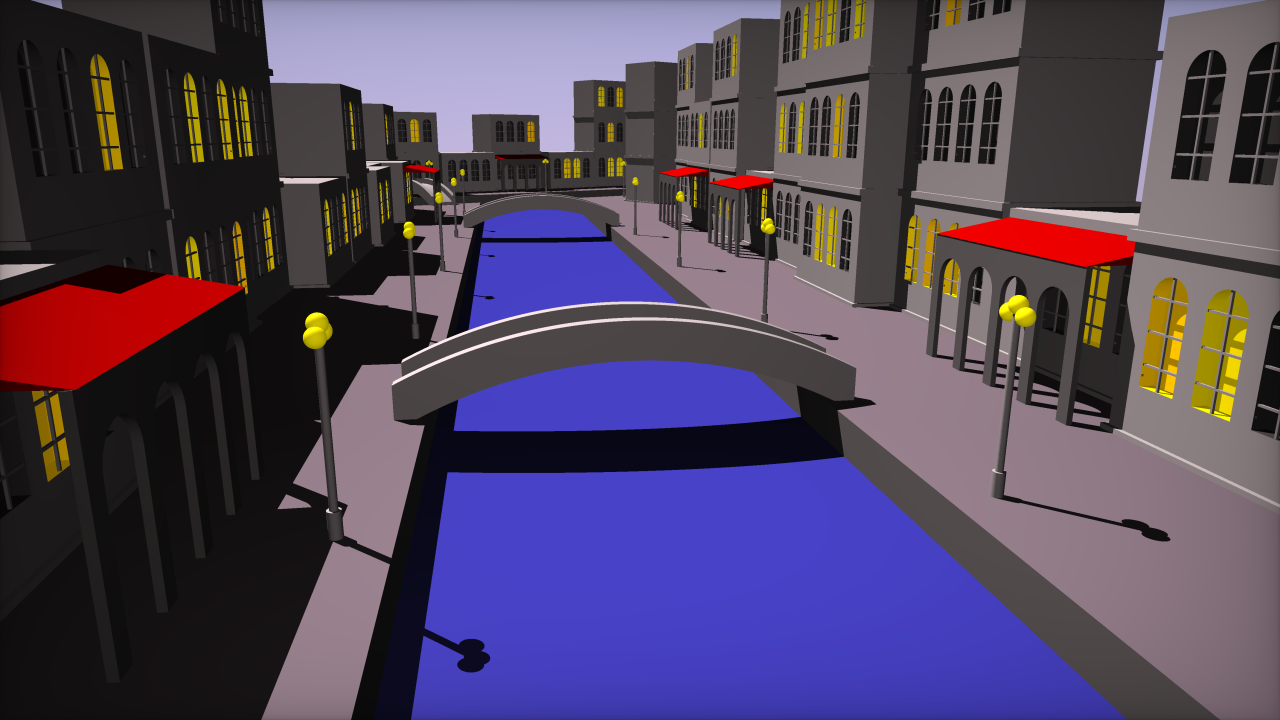
\includegraphics[width=0.95\linewidth]{screenshot_41} \\ а)
  \end{minipage}
  \hfill
  \begin{minipage}[ht]{0.49\linewidth}\centering
    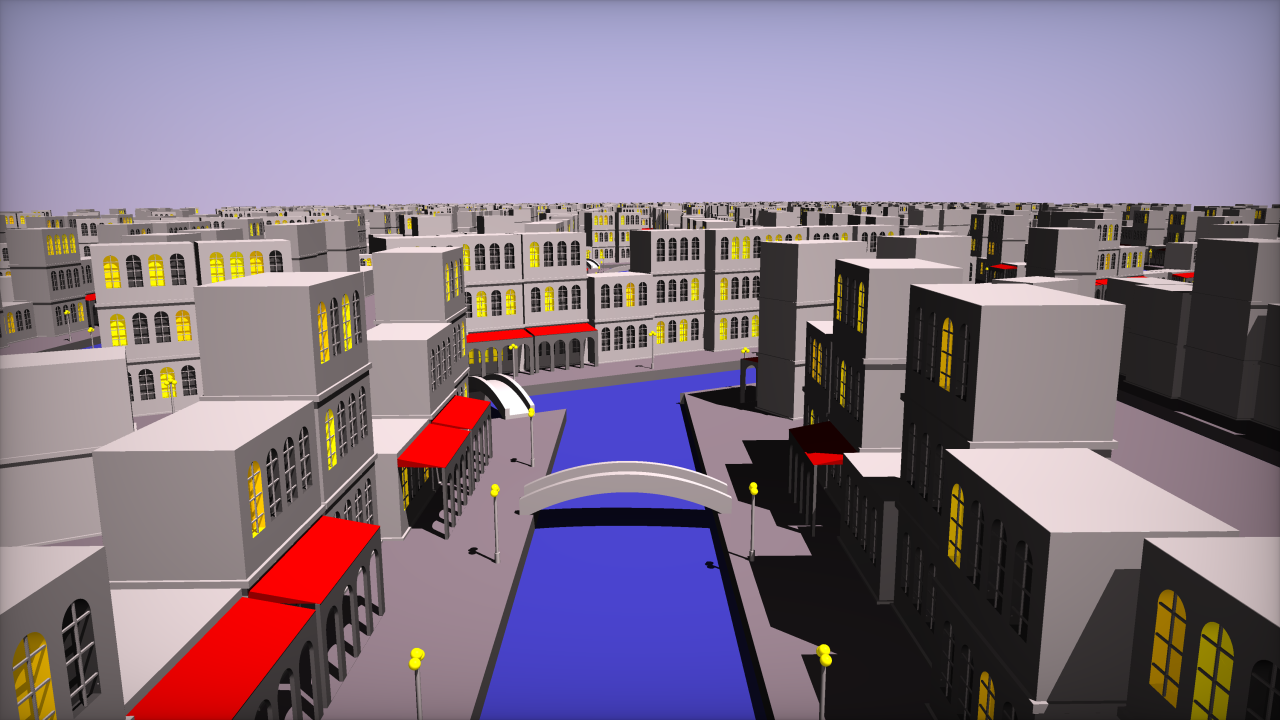
\includegraphics[width=0.95\linewidth]{screenshot_27} \\ б)
  \end{minipage}

  \begin{minipage}[ht]{0.49\linewidth}\centering
    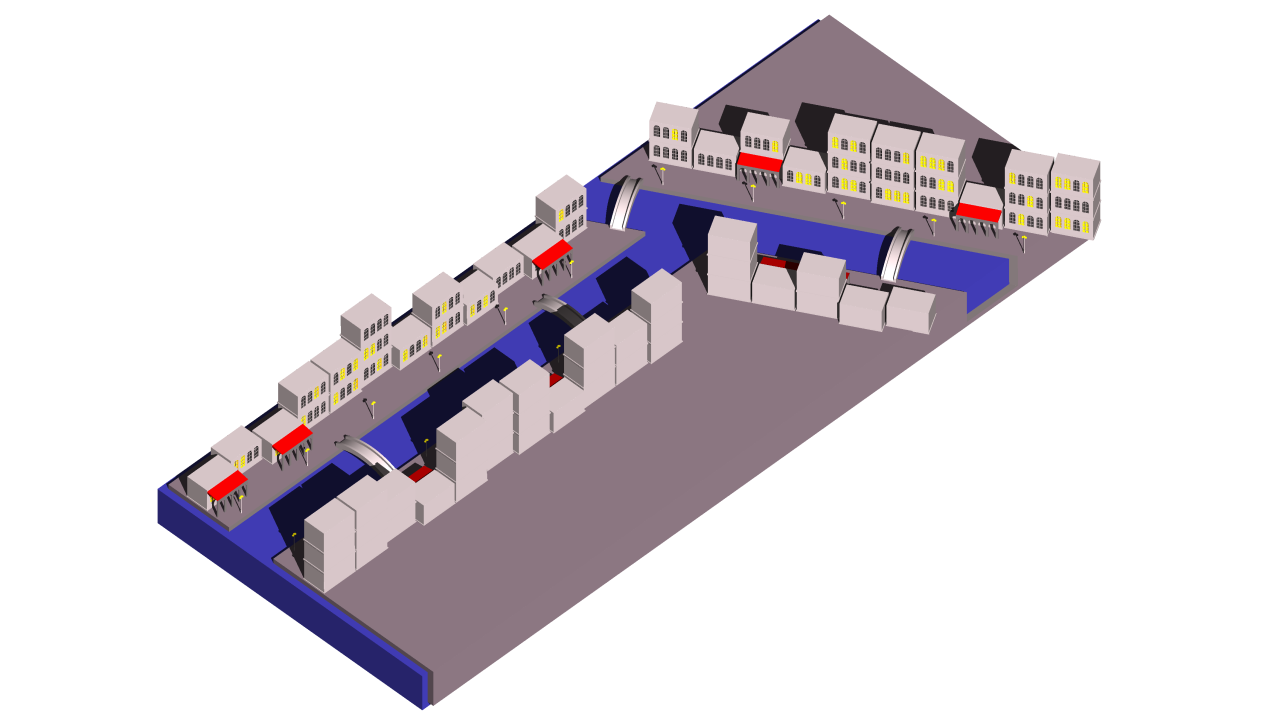
\includegraphics[width=0.95\linewidth]{screenshot_24} \\ в)
  \end{minipage}
  \hfill
  \begin{minipage}[ht]{0.49\linewidth}\centering
    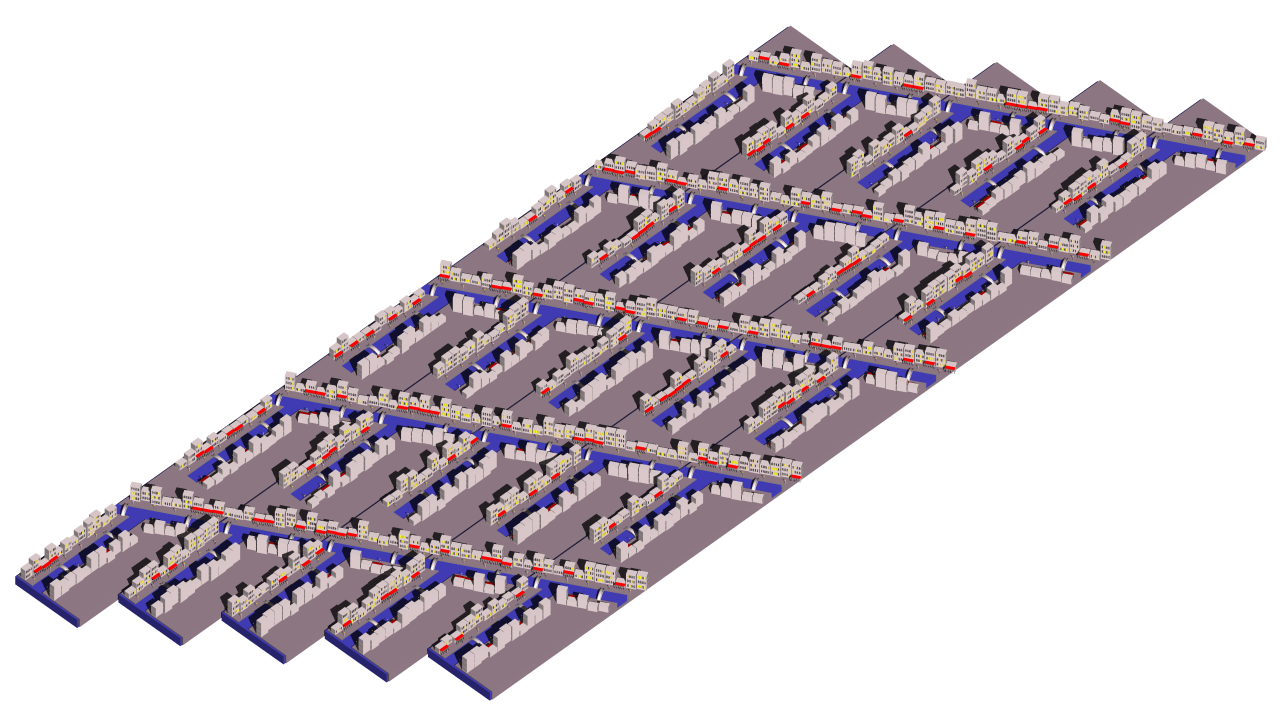
\includegraphics[width=0.95\linewidth]{screenshot_29} \\ г)
  \end{minipage}

  \begin{minipage}[ht]{0.49\linewidth}\centering
    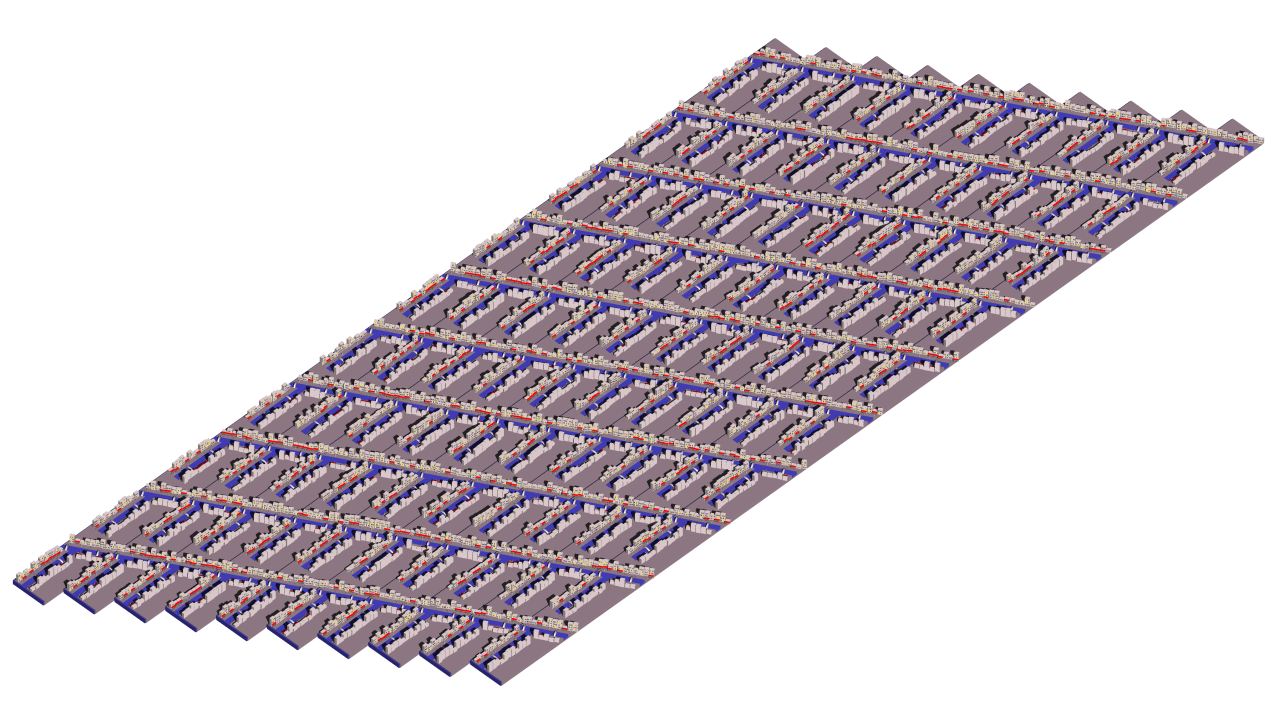
\includegraphics[width=0.95\linewidth]{screenshot_26} \\ д)
  \end{minipage}
  \hfill
  \begin{minipage}[ht]{0.49\linewidth}\centering
    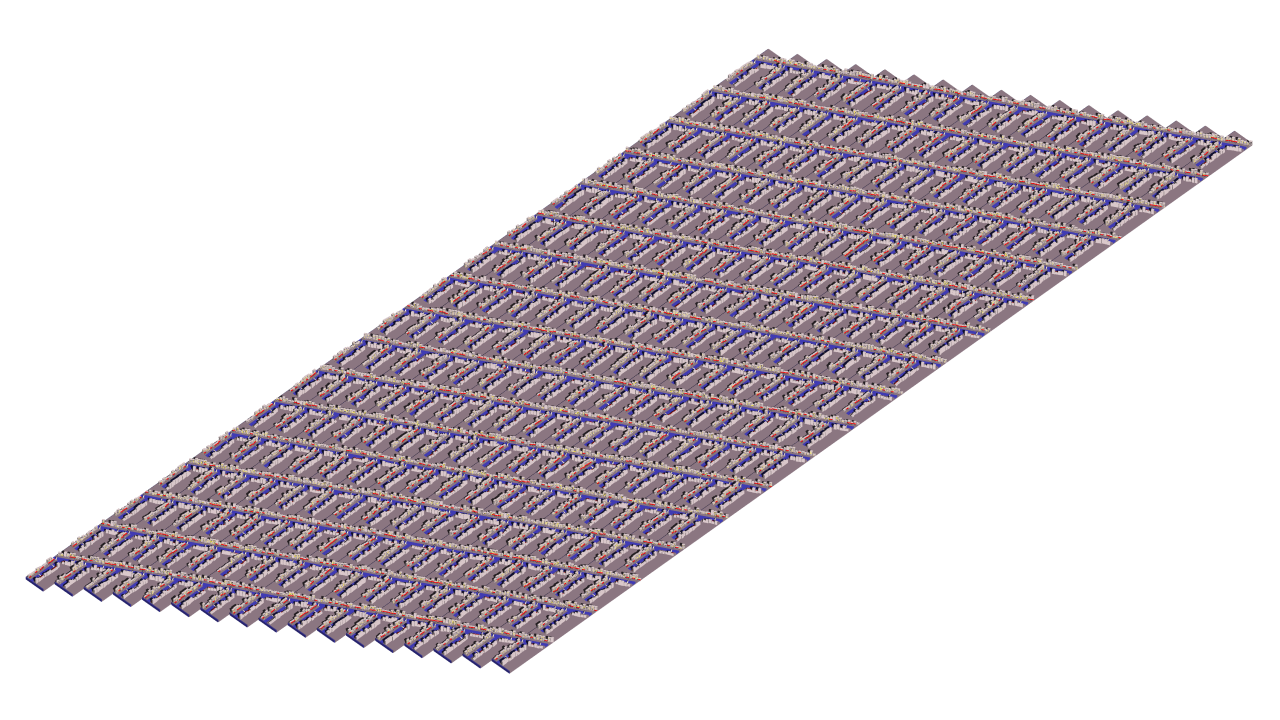
\includegraphics[width=0.95\linewidth]{screenshot_28} \\ е)
  \end{minipage}
  \caption{Сцена «Город»}
  \label{fig:results_city}  
\end{figure}

\begin{table} [ht]
    \caption{Оценки производительности}
    \label{tbl:timings}
    \begin{SingleSpace}
    \setlength\extrarowheight{5pt} %вот этим управляем расстоянием между рядами, \arraystretch даёт неудачный результат
    \setlength{\tymin}{1.9cm}% минимальная ширина столбца
    \begin{tabulary}{\textwidth}{@{}>{\zz}L >{\zz}C >{\zz}C >{\zz}C >{\zz}C >{\zz}C >{\zz}C >{\zz}C >{\zz}C@{}}
    	\toprule
		\multirow{3}{*}{Сцена} & \multirow{3}{*}{Примитивы} & \multirow{3}{*}{Глубина дерева} & \multicolumn{2}{c}{\textit{Int4000}} & \multicolumn{2}{c}{\textit{Rad7870}} & \multicolumn{2}{c}{\textit{GF680}}\\
		\cline{4-9}
		& & & $-$ & $+$ & $-$ & $+$ & $-$ & $+$\\
		\midrule
		Город (\textit{a}) & 3385   & 14 & 7   & 7.5 & 50  & 60 & 51  & 57\\
		Город (\textit{b}) & 343589 & 22 & 1.8 & 4.5 & 6.5 & 17 & 8   & 22 \\
		Город (\textit{c}) & 3385   & 14 & 21  & 22  & 66  & 68 & 120 & 125\\
		Город (\textit{d}) & 86673  & 20 & 8   & 11  & 21  & 25 & 31  & 38 \\
		Город (\textit{e}) & 343589 & 22 & 4.5 & 8   & 12  & 19 & 15  & 27 \\
		Город (\textit{f}) & 987218 & 24 & 2.3 & 7   & 6.7 & 18 & 8.3 & 21 \\

		\midrule

		Сыр (\textit{a}) & 1002  & 11 & 0.4        & 17  & 4.6        & 110  & 5.8        & 128\\
		Сыр (\textit{b}) & 8002  & 14 & \tiny{N/A} & 6.5 & 0.5        & 28   & 0.5        & 32 \\
		Сыр (\textit{c}) & 32002 & 17 & \tiny{N/A} & 0.5 & \tiny{N/A} & 3.7  & \tiny{N/A} & 4 \\

		\midrule

		Спутники (\textit{a}) & 87565   & 7 & 5    & 9    & 26  & 67  & 29  & 65 \\
		Спутники (\textit{b}) & 1120065 & 7 & 2.8  & 4.5  & 8   & 18  & 7  & 15 \\
		Спутники (\textit{c}) & 1120065 & 7 & 2.5  & 4.5  & 4.2 & 9   & 5.6 & 12 \\
		\bottomrule
    \end{tabulary}%
    \end{SingleSpace}
\end{table}

Вторая сцена для тестирования алгоритма представляет собой CSG модель «Швейцарского сыра» с дырами различного размера, смоделированными с помощью сфер (см. Рисунок~\ref{fig:results_cheese}). Число дыр возрастает с 1000 (а) до 8000 (б), и до 32000 (в) приводя к увеличению количества пересекающихся примитивов и сложности вычисления принадлежности точки определённой поверхности. В результате, производительность отрисовки модели «Швейцарский сыр» алгоритмом сильно зависит от успеха пространственной сортировки CSG дерева (см. Таблицу~\ref{tbl:timings}).

\begin{figure}[ht]
  \begin{minipage}[ht]{0.325\linewidth}\centering
    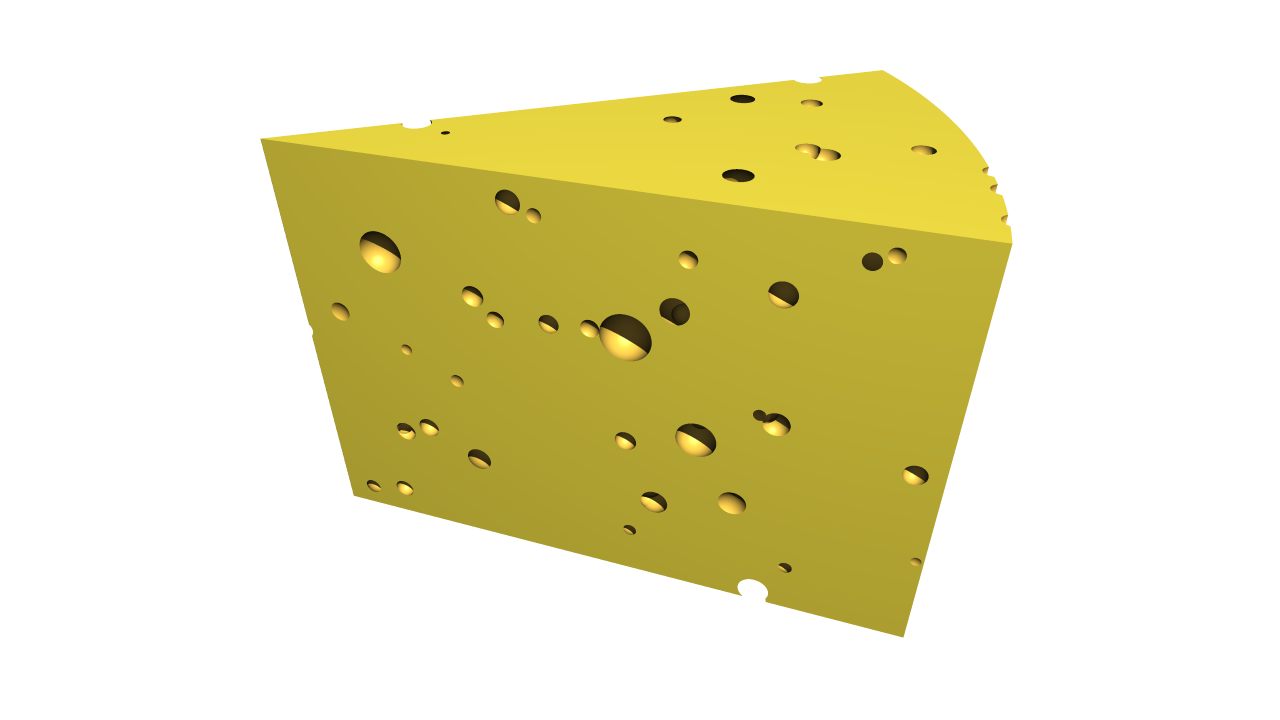
\includegraphics[width=0.95\linewidth]{screenshot_23} \\ а)
  \end{minipage}
  \hfill
  \begin{minipage}[ht]{0.325\linewidth}\centering
    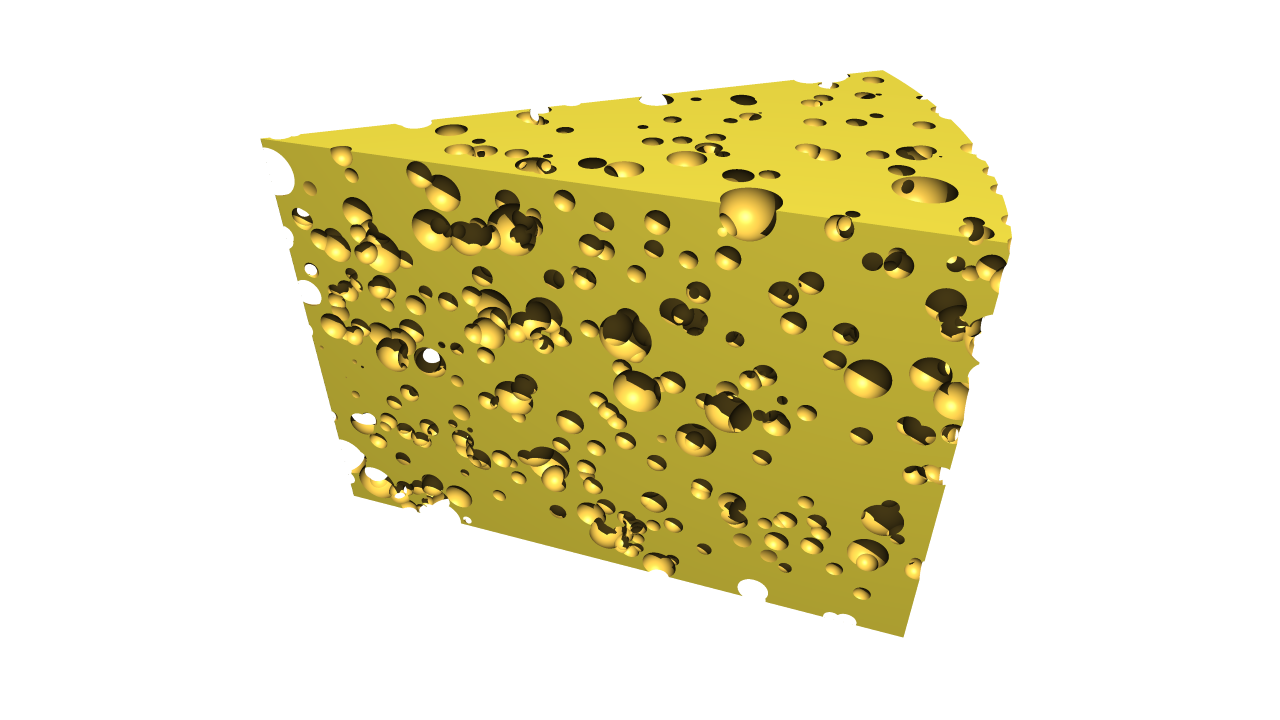
\includegraphics[width=0.95\linewidth]{screenshot_21} \\ б)
  \end{minipage}
  \hfill
  \begin{minipage}[ht]{0.325\linewidth}\centering
    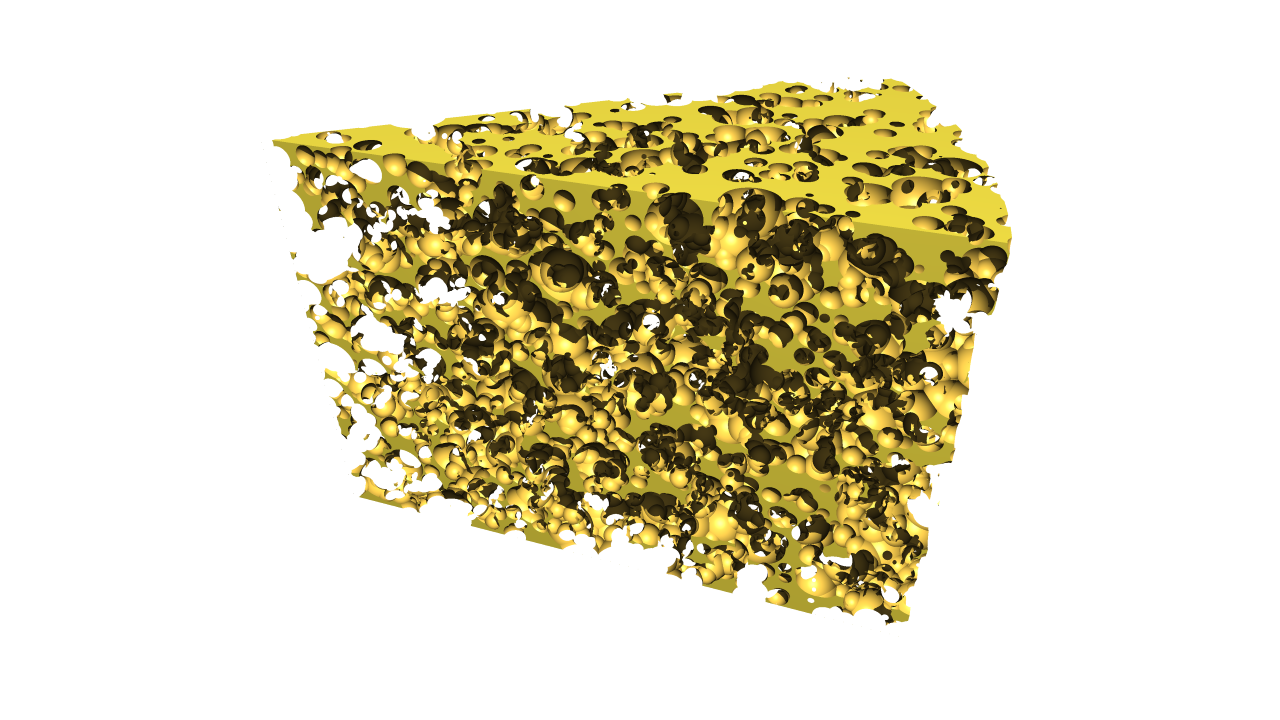
\includegraphics[width=0.95\linewidth]{screenshot_22} \\ в)
  \end{minipage}
  \caption{Сцена «Швейцарский сыр»}
  \label{fig:results_cheese}  
\end{figure}

\begin{figure}[ht]
  \begin{minipage}[ht]{0.325\linewidth}\centering
    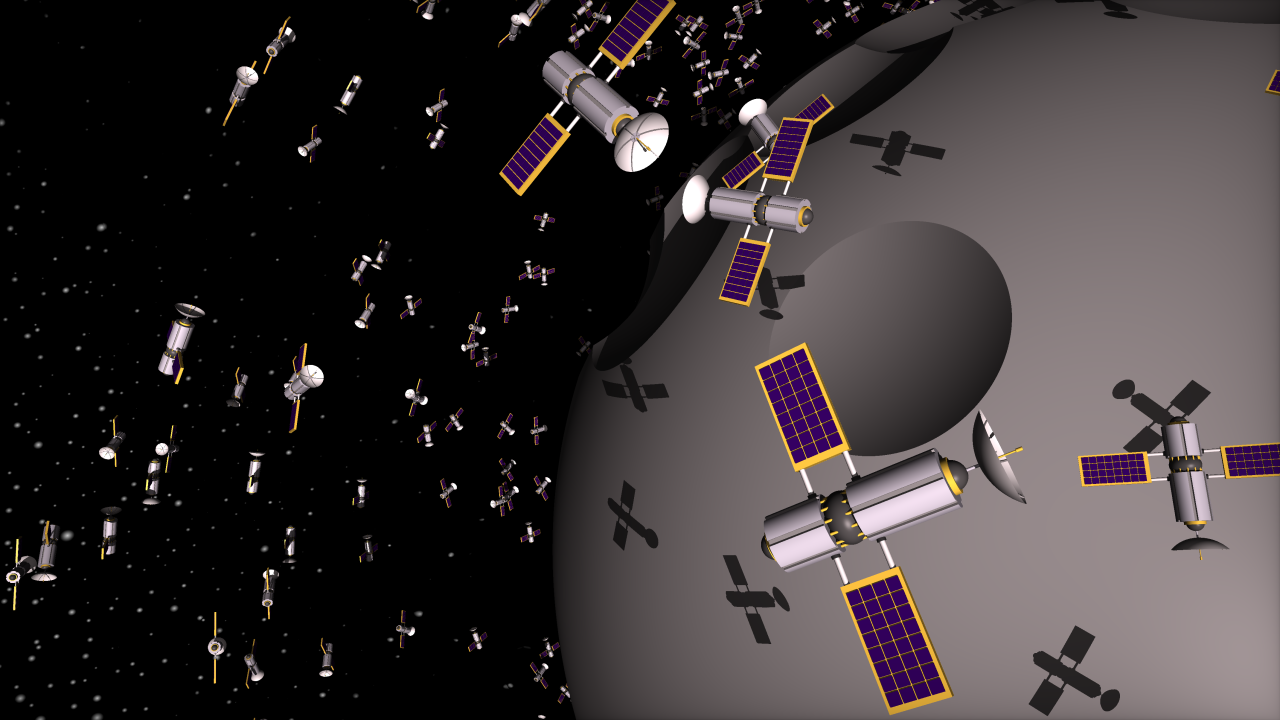
\includegraphics[width=0.95\linewidth]{screenshot_40} \\ а)
  \end{minipage}
  \hfill
  \begin{minipage}[ht]{0.325\linewidth}\centering
    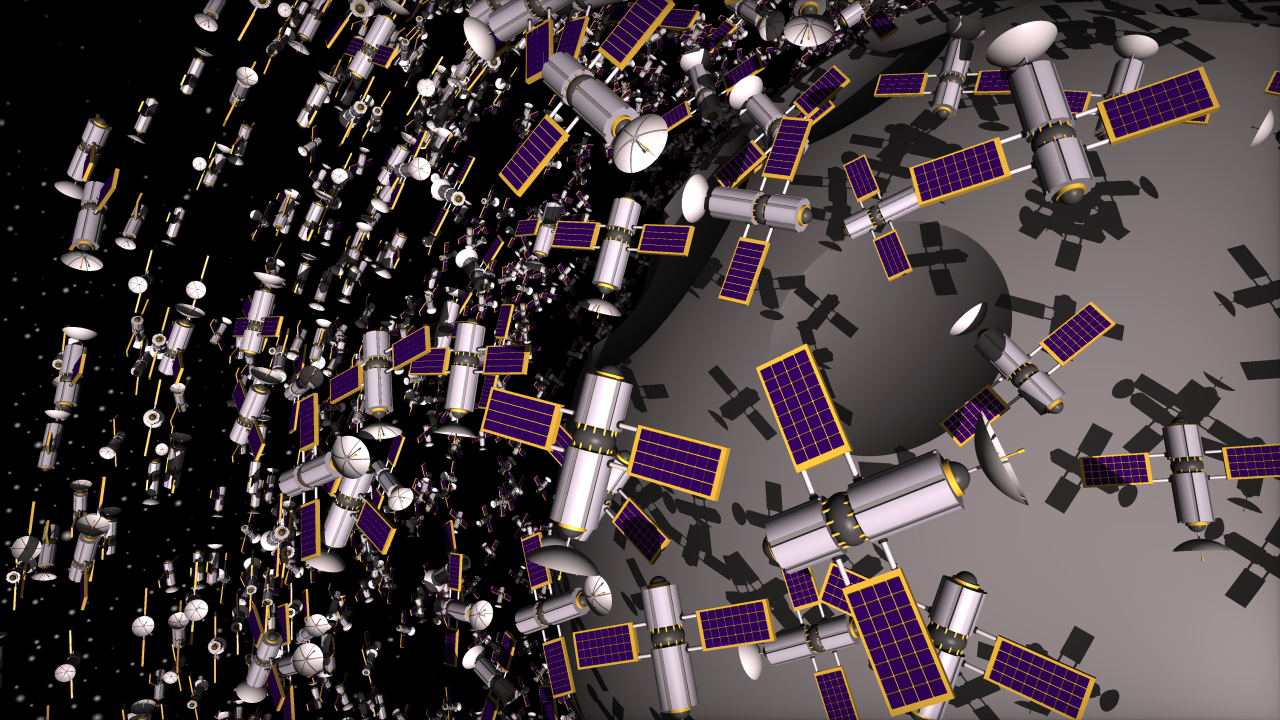
\includegraphics[width=0.95\linewidth]{screenshot_42} \\ б)
  \end{minipage}
  \hfill
  \begin{minipage}[ht]{0.325\linewidth}\centering
    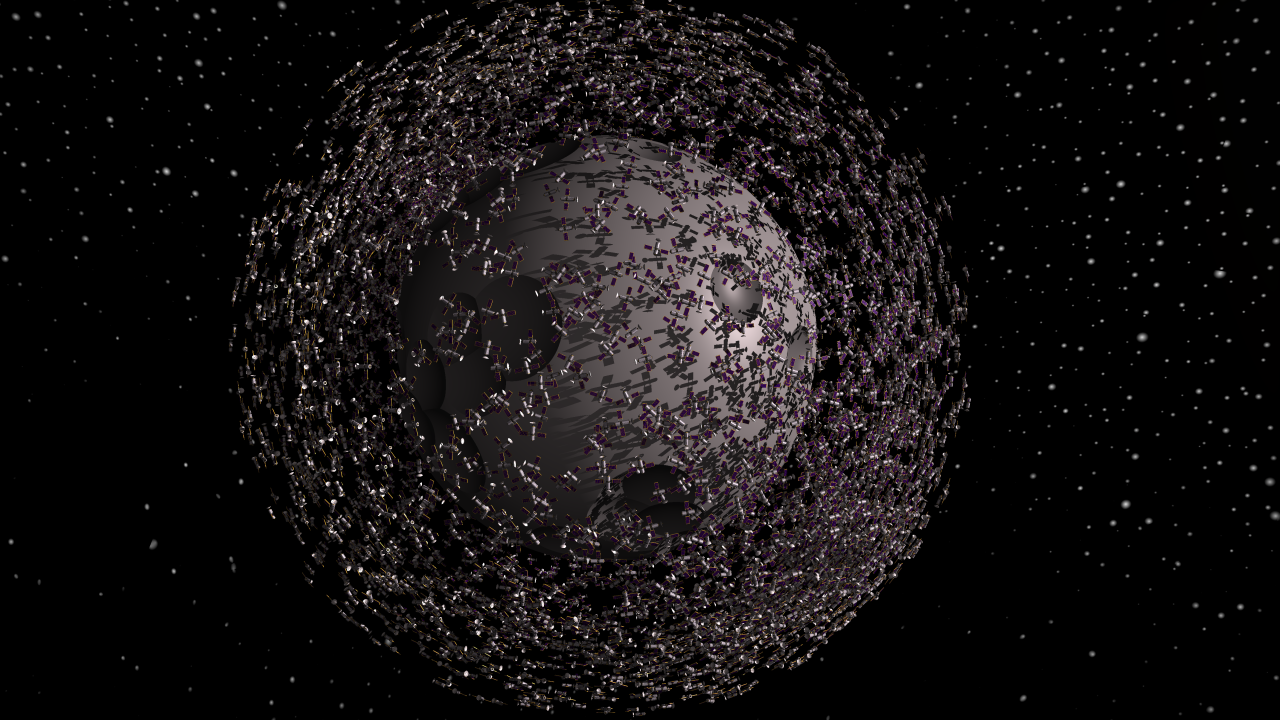
\includegraphics[width=0.95\linewidth]{screenshot_43} \\ в)
  \end{minipage}
  \caption{Сцена «Спутники» (варианты б и в отличаются только ракурсом)}
  \label{fig:results_sat}  
\end{figure}

Третья сцена демонстрирует спутники, вращающиеся вокруг планеты (см. Рисунок \ref{fig:results_sat}). В этой сцене, каждый спутник представлен отдельным CSG деревом. В рамках предложенного решения, набор независимых спутников присутствует в сцене как отдельные узлы BVH дерева верхнего уровня. В таком варианте представления сцены между отдельными спутниками невозможны Булевы операции, однако, так как все CSG деревья независимы, их изменения так-же могут быть независимыми. В то же время, благодаря быстрой процедуре перестроения BVH дерева верхнего уровня, взаимное положение спутников можно изменять динамически (например для анимации или для интерактивного редактирования сцены). Для измерения производительности такого подхода спутники движутся вокруг планеты по случайным круговым траекториям (см. Таблицу \ref{tbl:timings}).

В результате экспериментов, было обнаружено, что производительность предложенного решения линейно масштабируется с ростом тактовой частоты вычислительных ядер графического процессора (см. Рисунок \ref{fig:measurements}). Таким образом, предложенный алгоритм позволяет надеяться на дальнейший рост производительности по мере выхода новых поколений графических чипов. Тактовая частота памяти графического процессора, напротив, не влияет на производительность, что подтверждает предположение, что пропускная способность памяти не является главным ограничивающим фактором для предложенного алгоритма визуализации CSG моделей.

\begin{figure}[ht] 
  \centering
  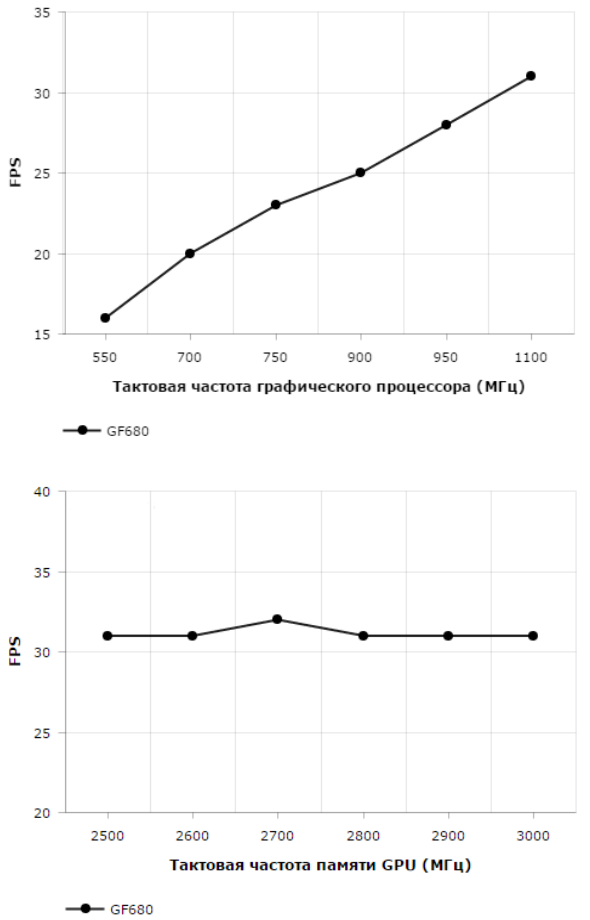
\includegraphics [scale=0.6] {measurements}
  \caption{Производительность на сцене «Швейцарский сыр» в зависимости от тактовой частоты (GF GTX 680)}
  \label{fig:measurements}
\end{figure}

Рассмотрим основные факторы, влияющие на производительность визуализации. Первым фактором, как и для всех методов, основанных на трассировке лучей, является разрешение экрана. Величина FPS меняется практически обратно пропорционально числу обработанных пикселей. Следующий важный фактор - это число примитивов в CSG модели, однако зависимость производительности от данного фактора сложнее. Эксперименты показывают, что, хотя визуализация сцены «Город», содержащей около миллиона CSG примитивов не вызывает затруднений, модель «Швейцарского сыра» показывает совершенно другие результаты. Такую разницу можно объяснить обширными перекрытиями примитивов в модели «Швейцарского сыра», которые заставляют алгоритм многократно проходить по CSG поддеревьям для однозначной классификации точек поверхности. Более того, из-за перекрытия ограничивающих объёмов также падает и эффективность пространственной сортировки узлов. Однако, даже на такой сложной сцене  алгоритм показывает зависимость производительности от числа примитивов близкую к линейной.

Представляет интерес сравнение производительности  GPU-реализации предложенного алгоритма с аналогами. Такое сравнение выполнено на наиболее сложном для алгоритма примере с «сыром» (табл. \ref{tbl:comparison}), в котором производительность аналогов превышена в 5 и более раз.

\begin{table} [htbp]%
    \centering
	\caption{Сравнение производительности (в FPS на GF GTX 680) с решениями-аналогами OpenSG и IceSL \todo{ours[7]}}%
	\label{tbl:comparison}
    \renewcommand{\arraystretch}{1.5}
    \begin{SingleSpace}
	\begin{tabular}{@{}@{\extracolsep{20pt}}llll@{}}
        \toprule
    	Сцена	& Предложенное решение & OpenSG	& IceSL	\\
        \midrule 
    	Сыр 1K 	& 128 	 & 2.1		& 1.1		\\
    	Сыр 8K	& 32 	 & 6.5		& 0.3		\\
    	Сыр 32K	& 4 	 & $\sim\!0$ & $\sim\!0$		\\
        \bottomrule
	\end{tabular}%
   	\end{SingleSpace}
\end{table}

Так как предложенное решение основано на трассировке лучей, оно было дополнено для поддержки визуальных эффектов глобального освещения, таких как прозрачность, мягкие тени, отражения, преломления и т.д (рис.~\ref{fig:photorealistic1}, рис.~\ref{fig:photorealistic2}).

\begin{figure}[ht] 
  \centering
  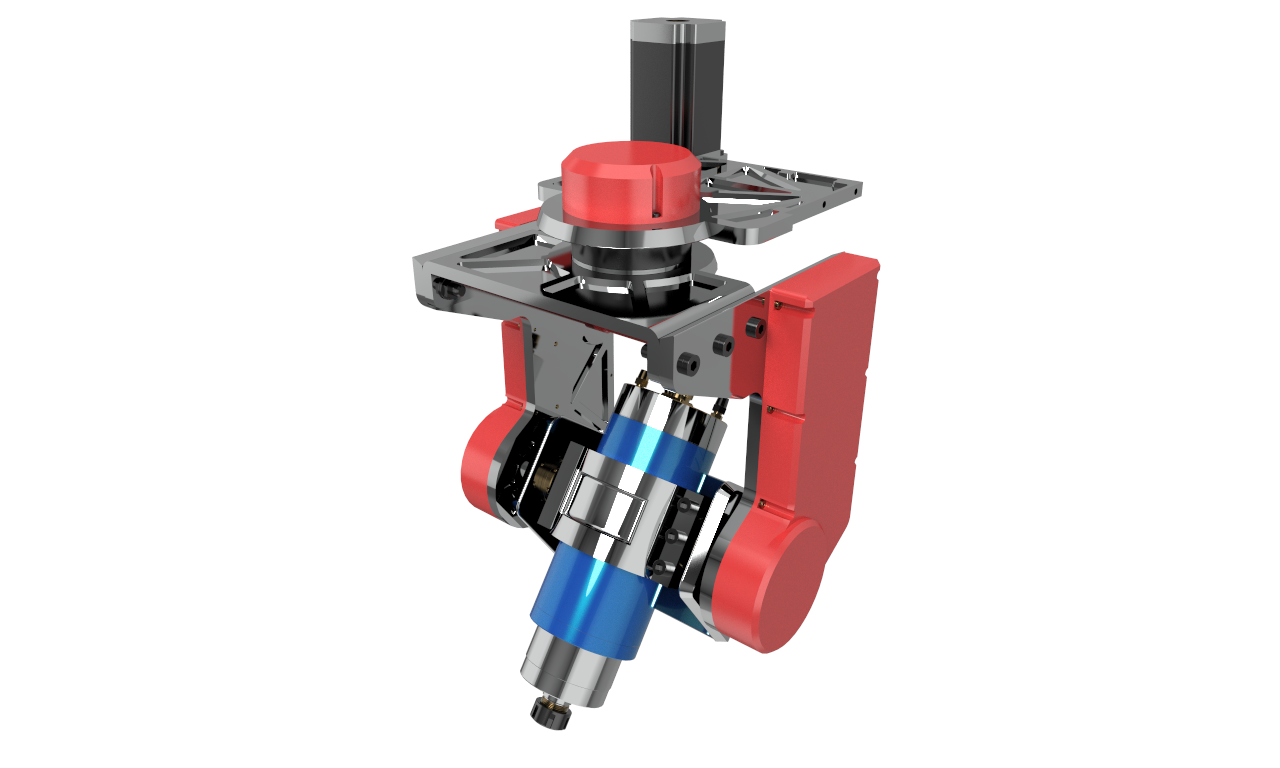
\includegraphics [scale=0.4] {2axis_milling}
  \caption{Фотореалистичная визуализация CSG модели 2-осевой фрезерной головки (построена на основе модели Tamas Cserto)}
  \label{fig:photorealistic1}
\end{figure}

\begin{figure}[ht] 
  \centering
  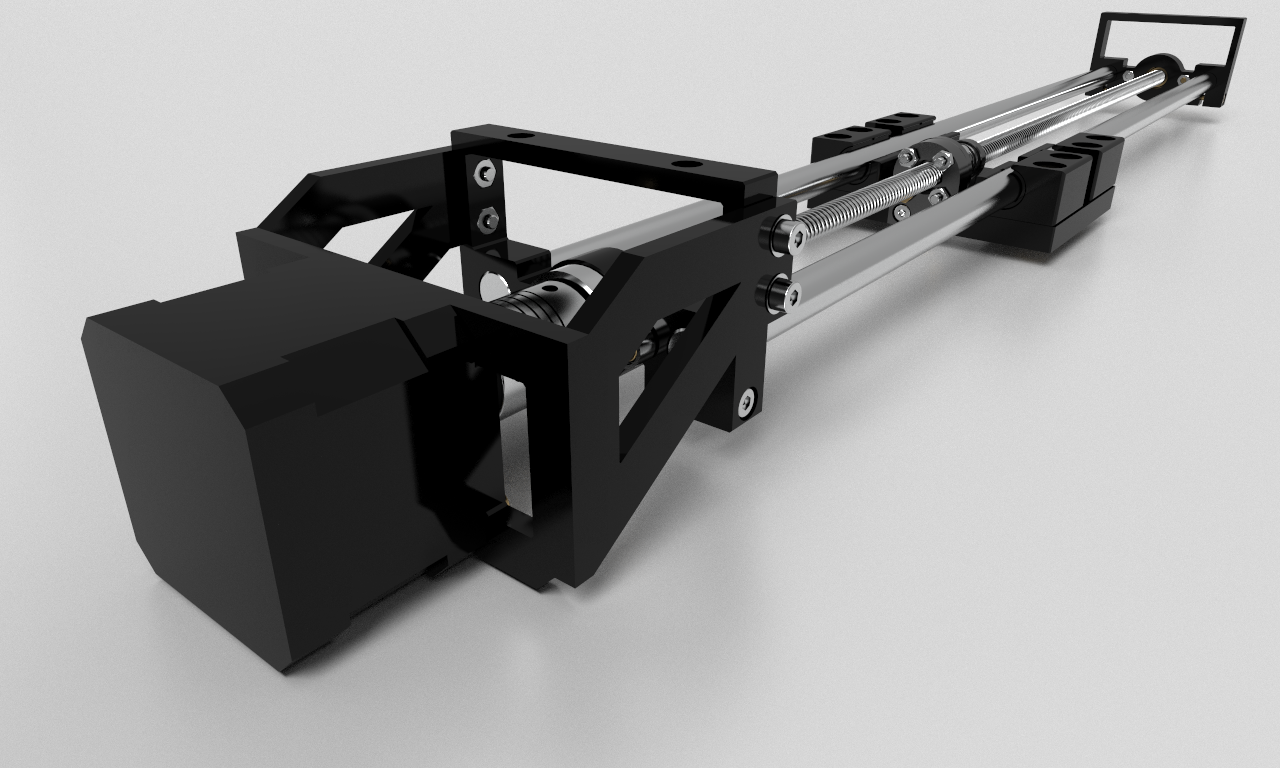
\includegraphics [scale=0.4] {linear_actuator}
  \caption{Фотореалистичная визуализация CSG модели линейного привода (построена на основе модели Aleksej Kolenčenko)}
  \label{fig:photorealistic2}
\end{figure}

Для полноценного включения визуализации CSG-моделей трассировкой лучей в САПР было обеспечено включение результата трассировки в стандартный конвейер растеризации 3D сцен, реализуемый OpenGL/GLSL. С этой целью, используя матрицу проецирования, для каждого луча вычисляется глубина точки пересечения очередного фрагмента, которая затем записывается в буфер глубины OpenGL. В результате визуализация CSG модели может быть дополнена произвольным текстом, линиями осей, сетками либо произвольными триангулированными объектами, отрисованными с помощью OpenGL.